\documentclass[a4paper,twoside]{article}

\usepackage[utf8]{inputenc} 
\usepackage[english]{babel}
\usepackage{graphicx}

\usepackage{cite}
\usepackage{color}
\usepackage{url}
\usepackage{hyperref}

\usepackage{subcaption}

\usepackage{xspace}
\usepackage{tikz}
\usepackage{stmaryrd}
\usepackage{bigstrut}
\usepackage{multirow}
\usepackage{epsfig}
\usepackage{stfloats}

%\usepackage{subfigure}
\usepackage{calc}
\usepackage{amssymb}
\usepackage{amstext}
\usepackage{amsmath}

\usepackage{amsthm}

\usepackage{multicol}
\usepackage{pslatex}
\usepackage{apalike}

\usepackage{macro}

\usepackage{SCITEPRESS}     % Please add other packages that you may need BEFORE the SCITEPRESS.sty package.

%\subfigtopskip=0pt
%\subfigcapskip=0pt
%\subfigbottomskip=0pt



\begin{document}

%
\title{Pattern Matching in discrete Models for Ecosystem Ecology}

\author{\authorname{Cinzia Di Giusto\sup{1}, Cédric Gaucherel\sup{2}, Hanna Klaudel\sup{3} and Franck Pommereau \sup{3}}
\affiliation{\sup{1}Université Côte d'Azur,  CNRS, I3S, France}
\affiliation{\sup{2}AMAP - INRA, CIRAD, CNRS, IRD, Université Montpellier,  France}
\affiliation{\sup{3}IBISC, Univ Evry,  Université Paris-Saclay, Evry, France}
\email{cinzia.di-giusto@univ-cotedazur.fr, cedric.gaucherel@cirad.fr,  \{hanna.klaudel, franck.pommereau\}@univ-evry.fr}
}

\keywords{Rewriting systems, similarity rate, pattern matching, ecosystems}


\abstract{
This paper studies models of ecosystems viewed as collections of interacting living (animals, plants, \ldots) and nonliving entities (air, water, soil, \ldots), whose conditions of appearance/disappearance are controlled by  sets of rules. 
We present a rule-based method allowing to automatically detect patterns (i.e., ecological processes) in ecosystems. The method relies on a measure of similarity and on an optimization algorithm. 
}

\onecolumn \maketitle \normalsize \vfill

\section{\uppercase{Introduction} }

Ecosystems are defined by complex processes of highly different nature: \eg bio-ecological, physico-chemical and socio-economical. 
The dynamics of such systems is difficult to grasp as it is the result of an intricate interplay between a large number of processes: the functioning of living species (fauna and flora) and the dynamics of soil and climate. 
In addition, all these entities and processes are influenced and often highly impacted by human activities. 
%
Understanding the functioning of ecosystems is, thus, crucial for a more sustainable management of them. 
Unfortunately, in practice, the study and management models of ecosystems are difficult. 
They are usually developed on a case-by-case basis due to the large number and continuous nature of variables. 
Here is a critical bottleneck, as we face today fast and dangerous changes of most ecosystems (due to climate change, impacting human activities, etc.) that we are compelled to understand so to properly react.

One way of improving our understanding of ecosystems functioning  is to provide more formal frameworks. 
They have proven to be valuable for speeding up and better controlling the decision procedures. 
%	
Similarly to what happens in biology, ordinary differential equations (ODE) are the dominant modeling methodology for ecosystems \cite{may72, Lotka1925}. 
The drawbacks of such  models are that: i) they usually need to quantify various parameters (mostly unknown). ii) They are not able to faithfully represent the time scale required for observation of ecological processes which is usually large. 
iii) On top of this,   analytic solutions usually do not exist and models often represent averaged and sometimes unrealistic behaviors of ecosystems. 
In contrast, while discrete models are high level abstractions of real life processes, they allow unraveling the tangled causal relationships between system's entities. 
The success of discrete approaches is witnessed, for instance,  in systems biology with formalisms like Petri
 nets~\cite{DBLP:journals/nc/BaldanCMS10}, Boolean networks~\cite{thomas1973boolean},
 process algebras~\cite{journals/tcsb/Cardelli05} and rewriting systems~\cite{giavitto04a}, to cite a few. 

%HK à relire
In ecology, discrete modelling is still pioneering and under exploited. 
Approaches such as \cite{gaucherel2012,gaucherel2014}, where the authors study the driving rules needed to change agricultural mosaics and model contrasted landscapes, are promising. However, much more may be obtained
by developing original solutions based on the suitable application of existing theory and associated (automated) tools. 
One of the goals of this paper is to contribute in this regard. 

As a starting point of our developments we take a general discrete formalism proposed in   \cite{pommereau-gaucherel2017}. Ecosystems are modeled qualitatively as a set of (living and nonliving) entities together with a set of rewriting rules expressing the conditions of their appearance/disappearance (\ie the ecosystem component behaviors).  
These rules  may be interpreted as the functioning bricks of landscape modelling. 
Each rule is, thus, part of a broader process describing the behavior of the full ecosystem. 

It is known that there are processes that are common to several ecosystems: \eg predation, competition, symbiosis, etc. and it is important to be able to identify them. In other words we can raise the following questions: how can we discover if a process is present in an ecosystem? is the introduction of a new entity causing the appearance of a known process? 
Indeed, discovering wanted or unwanted interaction patterns would guide decisions for taking actions according to the managing objectives, such as  preventing or reinforcing some ecosystemic functioning. 
Identify ecological processes or  \emph{interaction patterns} --in a more computer science oriented terminology--  by employing classical graph-theoretical methods on the state space is ineffective. 
Indeed, in realistic models, the ecosystem's dynamics usually leads to huge state spaces (often hundreds of thousands states). 
However, we can  search for  patterns only referring to the syntactical systems specification as it turns out that similar processes look similar at the rule level.  

From a more general point of view, a pattern search corresponds to a variant of the  problem of assessing the similarity between models of ecosystems. 
%
In order to compare two qualitative models of ecosystems, we introduce a pair of mappings, the first identifying entities and the latter rules, and a similarity measure expressed as a scoring function.  
This scoring majors the number of matched entities and rules, and penalizes those that do not perfectly match. 
Similarity is then defined as an optimization problem through the scoring function. The definition of the scoring function is used to search for interaction patterns in the rule-based models of ecosystems. 
As the complexity of this kind of search is exponential, it is not always possible in realistic cases to find optimal solutions. 
Nevertheless, optimization tools generally allow obtaining a sub-optimal solution quite efficiently, solutions that can then be refined. 

We implemented a prototype that allows encoding the matching of two models into a pseudo-Boolean optimization problem and calling tool Sat4j~\cite{sat4j} to solve it. 
We applied this prototype to systematically match a collection of interaction patterns against a set of models of ecosystems coming from various sources. 
 
The paper is structured as follows: Section \ref{sec:ecosystems} introduces the formal modeling of ecosystems we have used and presents running examples. Section \ref{sec:similarity} defines similarity measures used to compare ecosystems and discusses possible extensions of them. 
Several comparisons between ecosystems are used as illustrations for the scoring function.
In Section \ref{sec:experiments}, we present the results of our main case study: a research of interaction patterns in realistic ecosystems. %CG 
Section \ref{sec:related} is devoted to an overview of related work, while some concluding remarks and perspectives are presented in Section \ref{sec:conclusion}.  


\section{\uppercase{Ecosystems}}
\label{sec:ecosystems}
In this section, we recall the formal definition of a model of an ecosystem as given in \cite{pommereau-gaucherel2017}. 
An ecosystem consists in a set of \emph{entities} \E that can be present (\On) or absent (\Off). We assume that no entity may be simultaneously \On and \Off. The status (the presence) of an entity $a$ is called polarity, we use $a+$ to denote that $a$ is \On, $a-$ to denote that $a$ is \Off. The set of entities $\E$ with polarities $\mathsf{p} \in \{+,-\}$ is $\Ap= \{a+, a- \mid a \in \E\}.$ 
The presence of those entities is regulated by a sets of rewriting \emph{rules} \Ru.
More formally:

\begin{definition}[Ecosystem]
An \emph{ecosystem} \RR is a tuple \rsys{\E}{\Ru} such that:
\begin{itemize}
\item $\E$ is a set of entities, 
\item \Ru is a set of rewriting rules of the form
$ r: \rrule{\alpha^+}{\alpha^-}{\omega^+}{\omega^-}, $
where 
$r$ is the name of the rule, 
$\alpha^+$ and $\omega^+$ are sets of entities that are \On, and 
$\alpha^-$ and $\omega^-$ are sets of entities that are \Off.
\end{itemize}
\end{definition}

We denote by $\lhs{r}$ (respectively $\rhs{r}$) the set of entities in the left (respectively right) hand side of the rule $r$. 

An ecosystem state $s$ is defined by the information 
about the presence or absence of all its entities. It is described as the set of entities that are currently \On: thus 
$s \subseteq  \E$, and we assume  that the remaining entities $\E \setminus s$ are \Off.

The dynamics of an ecosystem \rsys{\E}{\Ru} is parametric over its initial state $s_0$.  
It comprises all reachable states obtained by asynchronously applying the rules in {\Ru}, in a non-deterministic way.
A rule $r$ is enabled at a state $s$ if the rule's left hand side, i.e., $(\alpha^+, \alpha^-)$,
matches the entities defining $s$. 
It means that $\alpha^+\subseteq s$ and $\alpha^- \cap s=\emptyset$.
If it is the case, the rule may apply and 
a new state $s'$ is generated by updating $s$ according to the rule's right hand side: $s'=(s\setminus \omega^-)\cup \omega^+. $
 

\begin{example}[Pond] \label{ex:pond}
We  consider a toy-model of a pond populated with two species of fish, piscivorous and insectivorous ones. The pond behavior is described  by the following rules: 

\begin{enumerate}
\item %\rulesimple{P-}{PF-,IF- }: 
\emph{if the pond disappears, all fish species disappear too,}
\item %\rulesimple{Su+}{P- }: 
\emph{in summer the pond dries and disappears,} 
\item %\rulesimple{P+}{PF+,IF+ }: 
\emph{if the pond is not dried, both species of fish may live in it,} 
\item %\rulesimple{PF+}{IF- }:
\emph{if the piscivorous fish are present, insectivorous fish disappear,}
\item %\rulesimple{IF-}{PF- }: 
\emph{if insectivorous fish disappear, piscivorous fish disappear too.}
\end{enumerate} %CG 

 It consists of four entities: the summer, the pond, and two kinds of fish (piscivorous and insectivorous); and seven rules (see Table \ref{tab:pond}): Rules 1--5 correspond to items 1--5 above, and rules 6 and 7 are used to simulate the change of the seasons.
\begin{table}[t]
\centering
\begin{tabular}{lll}
entities:&& \\
    &Su: &Summer \\
    &P: &Pond \\
    &PF: &Piscivorous Fish  \\
    &IF: &Insectivorous Fish
\end{tabular} \qquad 
\begin{tabular}{lll}
rules:&& \\
    &1: P$-$ & $\gg$ PF$-$, IF$-$  \\
    &2: Su+ &$\gg$  P$-$  \\
    &3: P+  &$\gg$ PF+, IF+  \\
    &4: PF+ &$\gg$ IF$-$  \\
    &5: IF$-$ &$\gg$ PF$-$ \\
    &6: Su+ &$\gg$ Su$-$ \\
    &7: Su$-$ &$\gg$ Su+ 
\end{tabular}
\caption{Entities and Rules for Example \ref{ex:pond}}\label{tab:pond}
\end{table}

As an example of the dynamics, let $s_0=\{$P$\}$ be the initial state. Then rule 3 is enabled and its application gives $s'=\{$P$, $IF$, $PF$\}$.
The whole dynamics is then a directed graph whose vertices are the reachable states and whose edges correspond to the application of rules.
\hfill $\diamond$
\end{example}

\begin{example}[Pesticides]\label{ex:pests}
As a second small example, consider a fragment of another ecosystem with four entities: birds, insects, pesticides and rain.

\begin{table}
\centering
\begin{tabular}{lll}
entities:&&\\
    &B: &Birds \\
    &I: &Insects \\
    &Pe: &Pesticide \\
    &R: &Rain \\
\end{tabular} \qquad
\begin{tabular}{lll}
rules :&&\\
    &1': B+ & $\gg$  I$-$  \\
    &2': I$-$ & $\gg$ B$-$ \\
    &3': Pe$-$, R+  & $\gg$ I+ \\
    &4': Pe+ & $\gg$ I$-$ \\
    &5': R+ & $\gg$ Pe$-$ \\
    &6': B$-$, Pe$-$ & $\gg$ I+ 
\end{tabular}
\caption{Entities and Rules for Example \ref{ex:pests}}\label{tab:pest}
\end{table}
The ecosystem is governed by the following principles: birds eat insects and if insects disappear, birds will vanish as well. As a disturbing factor we add pesticides that may kill insects. 
Pesticides are washed away by the rain and when there are no pesticides and it is still raining, insects proliferate. Similarly insect proliferation happens when there are no pesticides and no birds. 
We do not take into account in this example, all the rules (and possibly entities) that are necessary to regulate the presence/absence of rain.
Entities and rules are given in Table \ref{tab:pest}.
\hfill $\diamond$
\end{example}


%%%%%%%%%%%%%%%%%%%%%%%%%%%%%%%%%%%%%%%%%%%%%%%%%%%%%%%%%%%%%%%%%%%%%%%%%%%%%%
\section{\uppercase{Similarity between ecosystems}}
\label{sec:similarity}

As mentioned in the introduction, our objective is to identify interaction patterns.
An interaction pattern can be considered as a ``tiny" ecosystem restricted to few entities and rules. 
Thus it may be formalized in the same syntax as the one for the whole ecosystem. 
For example, the ``habitat" interaction pattern is composed of one entity featuring a specific environment (aquatic, terrestrial, pond,~\dots) and several entities inhabiting this environment: 
\begin{enumerate}
\item %\rulesimple{P-}{PF-,IF- }: 
\emph{if the environment disappears, all inhabitants disappear as well.}
\end{enumerate} 
%
Similarly, 
an interaction pattern for the ``predation" process is composed of two entities and two rules only:  
%
\begin{enumerate}
\item %\rulesimple{PF+}{IF- }:
\emph{if predators are present, then prey disappear,}
\item %\rulesimple{IF-}{PF- }: 
\emph{if prey disappear, then predators disappear too.}
\end{enumerate} 

In the example of the pond ecosystem, instances of both above patterns are present. The predation instance is composed of piscivorous and insectivorous species, and of rules 4 and 5; 
while the habitat instance is composed of entities pond, piscivorous and insectivorous species and of rule 1. 
Table \ref{tab:patt} shows a formal representation of the predation pattern.
%
\begin{table}
\centering
\begin{tabular}{ll}
entities:&\\
    &Pred: Predator \\
    &Prey: Prey \\
\end{tabular} \qquad 
\begin{tabular}{ll}    
rules:&\\
    &$1''$: Pred+  $\gg$ Prey$-$ \\
    &$2''$: Prey$-$  $\gg$ Pred$-$ \\~
\end{tabular}
\caption{Interaction pattern for predation pattern.}\label{tab:patt}
\end{table}
%
We may observe that there is a syntactical ``similarity" between rules 4 and 5 in the pond ecosystems and rules 1 and 2 in the predation pattern.

The concept of similarity will be the basis of our investigation.
Similarity  is discussed in theory (see for instance the philosophical work in \cite{tversky}) and also used in practice: in law \cite{Mooiman}, in nature sciences \cite{bbw090} and in 
various branches of computer science. 
Intuitively, we express it in terms of how many  groups of components with the same roles are present in both ecosystems.
%FP: isomorphes comment ? 
%HK c'est expliqué intuitivement dans la phrase plus bas :
This means that, given two mappings, between entities and rules respectively, 
the similarity rate is defined as the number of mapped entities plus how many mapped entities the rules have in common. 
More precisely, let $\RR_1 = \rsys{\E_1}{\Ru_1}$ and $\RR_2 =
\rsys{\E_2}{\Ru_2}$ be two ecosystems, and \mapcomp and \maprule be two mappings between entities and rules respectively.
The first one is $\mapcomp : \E^p_1 \to \E^p_2.$
%this means that, for instance, $a+ \in \E^p_1$ could be mapped into either $b+$ or $c-$  for  $b+,c- \in  \E^p_2$.  
The mapping \mapcomp is injective but not necessarily total and polarities are consistent: \ie if $a+$ is matched with $b-$ then $b+$ is matched with $a-$. It is encoded as a rectangular matrix $X$  of size $(|\E^p_1| \times |\E^p_2|)$ of Boolean values defined for each pair of entities with polarities $(m,n) \in \E^p_1 \times \E^p_2$ as
$$X_{m,n} = 1 \text{ if } \mapcomp(m)=n, 0 \text{ otherwise.} $$

In order to implement  injectivity and the correspondence between polarities we introduce three restrictions (see Figure~\ref{fig:matrix-match}): 
\begin{enumerate}
\item There is at most one ``1" in  each line:~ 
$$
\forall m \in \Ap_1: \quad
   \sum_{n \in \Ap_2} X_{m,n}  \leq 1;
  $$
  
 \item There is at most one ``1" in  each column:~  
$$
\forall n \in \Ap_2: \quad
   \sum_{m \in \Ap_1} X_{m,n}  \leq 1;
  $$
 \item Polarities are consistently matched: 
\begin{align*}
 &\forall a \in \E_1, b \in \E_2: \\
  & \quad X_{a+,b-} = X_{a-,b+} \land X_{a+,b+} = X_{a-,b-} .
\end{align*}
\end{enumerate}


\begin{figure*}[t]
\centering
\begin{subfigure}{0.4\textwidth}
  \begin{center}
    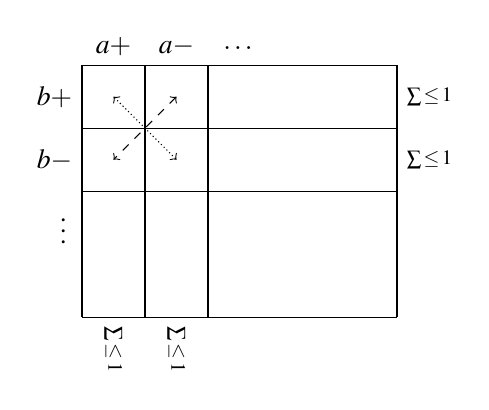
\begin{tikzpicture}[yscale=-1,scale=.8]
      \foreach \y in {0,1,2,4} {
        \draw (0,\y) -- (5,\y);
      }
      \foreach \x in {0,1,2,5} {
        \draw (\x,0) -- (\x,4);
      }
      \node[above] at (.5,0) {$a+$};
      \node[above] at (1.5,0) {$a-$};
      \node[above=2pt] at (2.5,0) {$\dots$};
      \node[left] at (0,.5) {$b+$};
      \node[left] at (0,1.5) {$b-$};
      \node[left=2pt] at (0,2.5) {$\vdots$};
      \node[right] at (5,.5) {$\scriptstyle{\sum}\,\leq\,{1}$};
      \node[right] at (5,1.5) {$\scriptstyle{\sum}\,\leq\,{1}$};
      \node[right,rotate=-90] at (.5,4) {$\scriptstyle{\sum}\,\leq\,{1}$};
      \node[right,rotate=-90] at (1.5,4) {$\scriptstyle{\sum}\,\leq\,{1}$};
      \draw[<->,densely dotted] (.5,.5) to node {} (1.5,1.5);
      \draw[<->,dashed] (1.5,.5) to node {} (.5,1.5);
    \end{tikzpicture}
  \end{center}
  \caption{The encoding into matrix $X$ of the mapping \mapcomp for entities and the illustration of corresponding restrictions.}
  \label{fig:matrix-match}
  \end{subfigure} \qquad \qquad 
  \begin{subfigure}{0.4\textwidth}
  \begin{center}
    \begin{tikzpicture}[yscale=-1,scale=.8]

        \foreach \y in {0,1,3} {
          \draw (0,\y) -- (4,\y);
        }
        \foreach \x in {0,1,4} {
          \draw (\x,0) -- (\x,3);
        }
        \node[above] at (.5,0) {$u_1$};
        \node[above=2pt] at (1.5,0) {$\dots$};
        \node[left] at (0,.5) {$v_1$};
        \node[left=2pt] at (0,1.5) {$\vdots$};
        \node[right] at (4,.5) {$\scriptstyle{\sum}\,\leq\,{1}$};
        \node[right,rotate=-90] at (.5,3) {$\scriptstyle{\sum}\,\leq\,{1}$};
 %     \end{scope}
    \end{tikzpicture}
  \end{center}
  \caption{The encoding of matrix $Y$ of the mapping $\maprule$ for the rules and the corresponding restrictions.}
  \label{fig:matrix-matchrule}
  \end{subfigure}
  \caption{Encoding of mappings \mapcomp and \maprule  }
\end{figure*}


Similarly, the mapping $\maprule: \Ru_1 \to \Ru_2$ maps the rules. As for entities, it is encoded as a rectangular matrix $Y$ of size $(|\Ru_1| \times |\Ru_2|)$ of Boolean values defined for each pair of rules $(u,v)\in \Ru_1 \times \Ru_2$  as
$$Y_{u,v} =1 \text{ if } \maprule(u)=v, 0 \text{ otherwise.}$$
It is subjected to the following restrictions that implements injectivity (see Figure \ref{fig:matrix-matchrule}):\looseness=-1
\begin{enumerate}
\item There is at most one ``1" in  each line:~
$$
 \forall u \in \Ru_1: \quad
   \sum_{v \in \Ru_2} Y_{u,v} \leq 1;
  $$
  
 \item There is at most one ``1" in  each column: ~ 
$$
  \forall v \in \Ru_2: \quad
  \sum_{u \in \Ru_1} Y_{u,v} \leq 1. 
  $$
\end{enumerate}

% \begin{figure}
%   \begin{center}
%     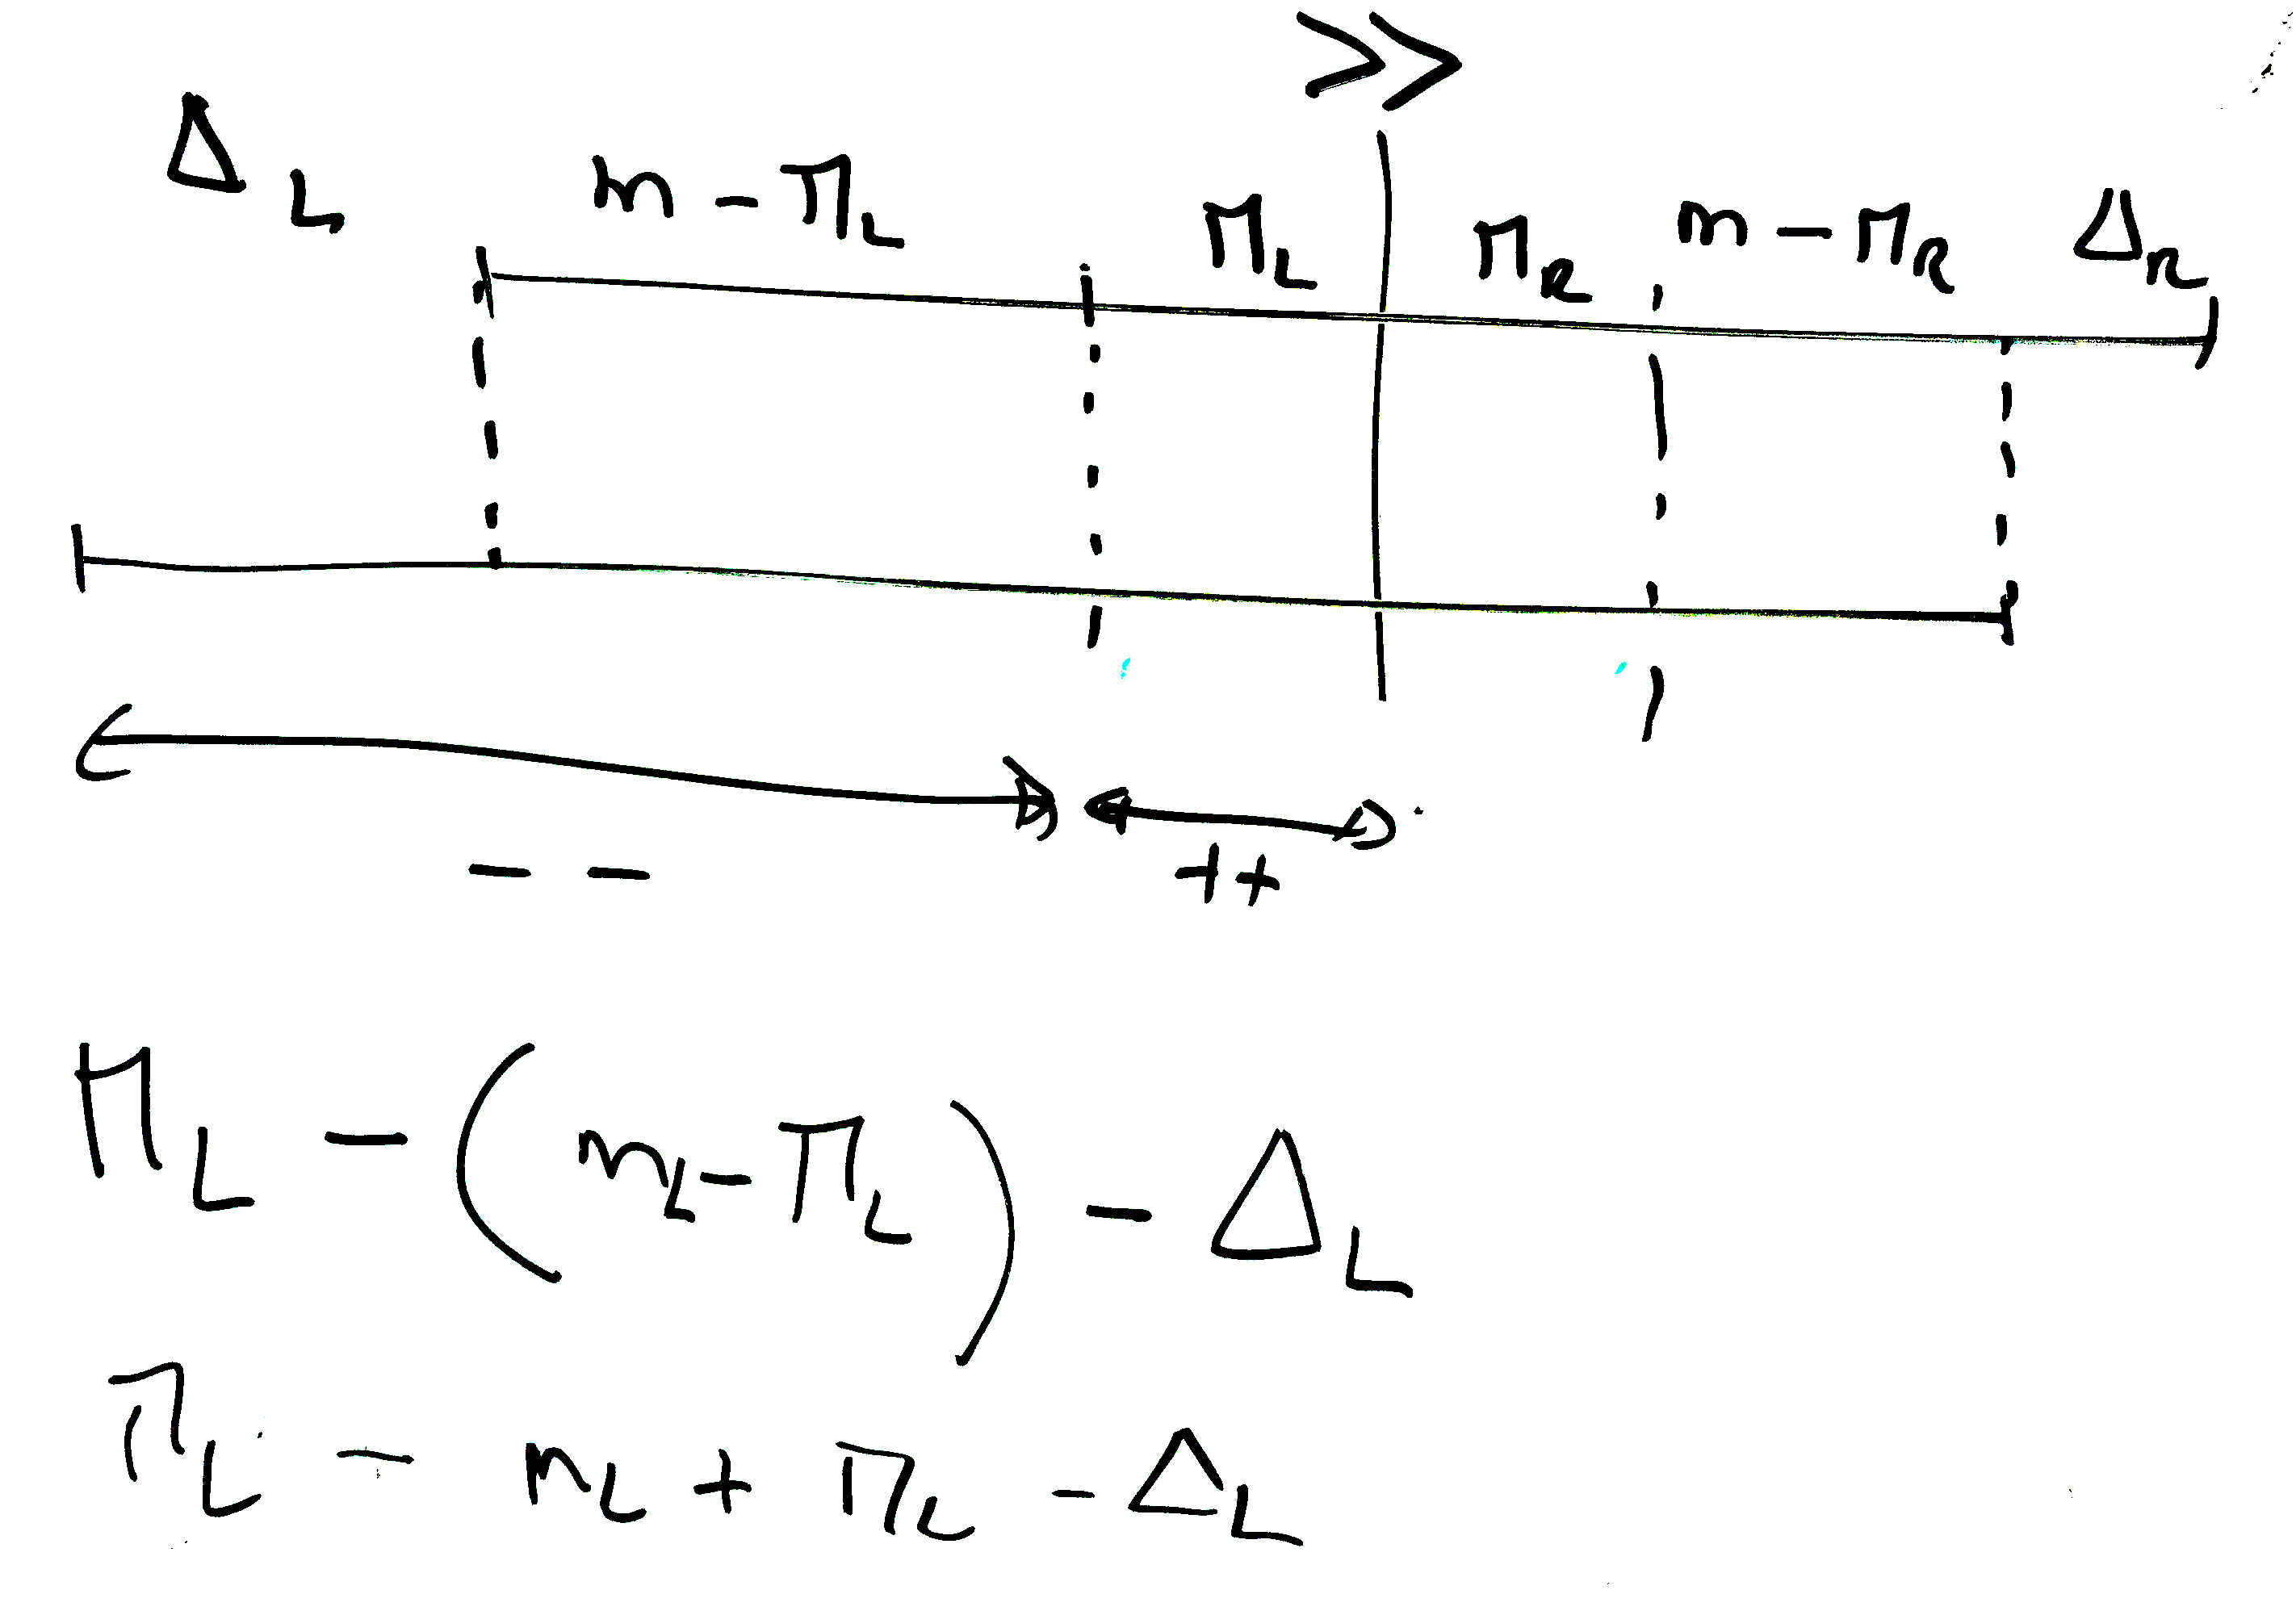
\includegraphics[width=\columnwidth]{score}
%   \end{center}
%   \caption{Intuition of the score function}
%   \label{fig:score-explained}
% \end{figure}

For each pair of mappings (\mapcomp,\maprule) between ecosystems $\RR_1$ and $\RR_2$ we define a \emph{scoring} function \gf.
The function assesses the quality of the matching rules with respect to the number of matching entities. 
The simplest way to express the score is to count,  for each pair of  matching rules  $\maprule(u) =v$ (\ie $Y_{u,v}=1$), the number of matching entities through  function \mapcomp on both the left and right hand side (\ie  for each pair of entities $n$ and $m$  in rules $u$ and $v$ respectively, we count the sum of all  $X_{n,m} =1$). 
The scoring function is a ratio between previous sum and a constant that counts the number of rules times  the maximal  number of entities in a  rule.
More precisely: 
$$  \gf_0(X,Y) = {}
   \frac{1}{\Ti\cdot \rulemax} \phantom{m} \cdot \sum_{\mathclap{\begin{array}{l} u \in \Ru_1, \\ v \in \Ru_2 \end{array}}}    \phantom{mm} \bigg( Y_{u,v} \cdot 
  \sum_{\mathrlap{n \in u, m \in v}} X_{n,m}
  \bigg) 
$$
where 
$ \rulemax = \min (|\Ru_1|, |\Ru_2|)$ 
is the cardinality of the set of rules in the ecosystem having the smallest number of them, and
$\Ti = \max_{u\in \Ru_1 \cup \Ru_2} (|\lhs{u}| + |\rhs{u}|)$
is the maximal number of entities in a rule in both ecosystems, considering at the same time the left ($\lhs{\cdot}$) and right ($\rhs{\cdot}$) hand side.
However this simple scoring does not take into account:
\begin{enumerate}
\item the different contribution of the left and right hand side. This means, for instance, that a good matching on the left hand side can compensate a bad matching on the right hand one; 
\item the proportion of entities that are not matched. Scoring function $\gf_0$ does not differentiate between two rule mappings  that for a rule in one ecosystem  match the same number of entities but the size of matched rules in the second system is different.
\end{enumerate}

\begin{example}
For example, take the ecosystems $\Ru_1$ with one rule ${r_1: A+, B+ \gg C+}$ and  $\Ru_2$ with two rules ${r_2: A+, B+ \gg C+}$ and ${r_3: A+, B+, D- \gg C+}$ .
The score for $\maprule_1$ mapping ${r_1}$ to ${r_2}$ should be greater than $\maprule_2$ mapping ${r_1}$ to ${r_3}$ as in the latter the mapping is less perfect and there are entities that are not matched.
\hfill $\diamond$
\end{example}


We thus propose a better formulation for the scoring function that takes into account these remarks.
The  scoring function is now the sum of the scores of the left hand side and the right hand side and can be summarized as follows:

\begin{align*} 
  \gf(X, Y) \defeq {} 
  %
  & \frac{1}{\rulemax \cdot (\Lhs + \Rhs) } ~\cdot \sum_{\mathclap{u \in \Ru_1, v \in \Ru_2}} Y_{u,v}  (\mathit{left}(u,v)+\mathit{right}(u,v) ) 
\end{align*}
%
where $\rulemax = \min (|\Ru_1|, |\Ru_2|)$ as above, 
$\Lhs =  \max_{u\in \Ru_1 \cup \Ru_2} (|\lhs{u}|)$ and 
$\Rhs = \max_{u\in \Ru_1 \cup \Ru_2} (|\rhs{u}|)$ 
%
% \begin{align*} 
% \rulemax = & \min (|\Ru_1|, |\Ru_2|) \mbox{ as above, }\\[4mm]
% 	\Lhs = & \max_{u\in \Ru_1 \cup \Ru_2} (|\lhs{u}|) \mbox{ and }\\[4mm]
%    \Rhs =  &\max_{u\in \Ru_1 \cup \Ru_2} (|\rhs{u}|)
% \end{align*}
 are the maximal numbers of entities occurring in the left (respectively right) hand side of the  rules from both ecosystems, and $ \mathit{left}(u,v)$ and  $\mathit{right}(u,v) $ are the scores for each pair of matching rules $u \in \Ru_1$ and $v \in \Ru_2$:

\begin{align*} 
   \mathit{left}(u,v) =  &
    \quad  \sum_{\mathrlap{\substack{n \in \lhs{u},\\ m \in \lhs{v}}}} X_{n,m} \\
          &- \bigg(\min(|\lhs{u}|, |\lhs{v}|) - \sum_{\mathrlap{\substack{n \in \lhs{u},\\ m \in \lhs{v}}}} X_{n,m} \bigg) \\
         & - \abs(|\lhs{u}| - |\lhs{v}|)   \\ 
    = & \quad 2 \cdot \sum_{\mathrlap{\substack{n \in \lhs{u},\\ m \in \lhs{v}}}} X_{n,m} 
         -\min(|\lhs{u}|, |\lhs{v}|) \\
        &- \abs(|\lhs{u}| - |\lhs{v}|)   \\[2mm]
   \mathit{right}(u,v) = & \quad 2 \cdot \sum_{\mathrlap{\substack{n \in \rhs{u},\\ m \in \rhs{v}}}} X_{n,m}
                  - \min(|\rhs{u}|, |\rhs{v}|) \\
                 & - \abs(|\rhs{u}| - |\rhs{v}|)   
\end{align*}


The construction of this scoring function is depicted in Figure~\ref{fig:scoring} below.
The part $\mathit{left}(u,v)$ takes the number of matching entities $$M_L=\sum_{\mathrlap{n \in \lhs{u}, m \in \lhs{v}}} X_{n,m}$$ and subtracts two penalties. The first one: $\min(|\lhs{u}|, |\lhs{v}|) - M_L$ corresponds to the maximum number of entities, which could be matched minus those that are actually matched. The second one: 
$\abs(|\lhs{u}| - |\lhs{v}|)$ expresses the number of entities which could never be matched because of the difference in the length of the left hand sides of  the two rules.
This score is maximal when $\mathit{left}(u,v) = \min(|\lhs{u}|, |\lhs{v}|) \text{ and } |\lhs{u}| = |\lhs{v}|,$ \ie the left hand sides of $u$ and $v$ have the same length, and all their entities match. 
The part for the right hand sides is defined analogously.
The overall score is normalized with respect to the number of rules $\rulemax$ times $\Lhs$ plus $\Rhs$. As an effect of penalties, the score can be negative but it is always between -1 and 1.


\begin{figure*}[t]
  \begin{center}
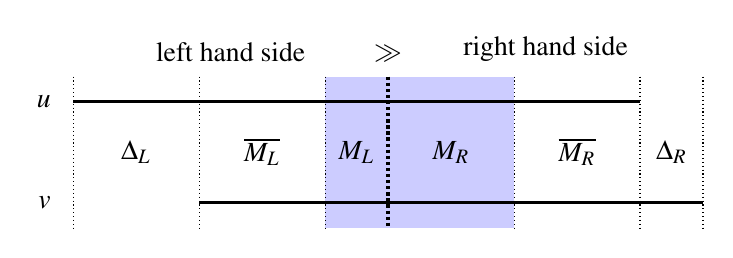
\begin{tikzpicture}[yscale=.8,scale=.8]

\fill[blue!20!white] (4,4.5) rectangle (7,1.5);

\draw[very thick] (0,4) -- (9,4);
\draw[very thick] (2,2) -- (10,2);

\node[left] at (-.2,4) {$u$};
\node[left] at (-.2,2) {$v$};

\node[above] at (2.5,4.6) {left hand side};
\node[above] at (7.5,4.6) {right hand side};
\node[above] at (5,4.6) {$\gg$};

\node at (1,3) {$\Delta_L$};
\node at (3,3) {$\overline{M_L}$};
\node at (4.5,3) {$M_L$};
\node at (6,3) {$M_R$};
\node at (8,3) {$\overline{M_R}$};
\node at (9.5,3) {$\Delta_R$};

\draw[densely dotted] (0,4.5) -- (0,1.5);
\draw[densely dotted] (2,4.5) -- (2,1.5);
\draw[densely dotted] (9,4.5) -- (9,1.5);
\draw[densely dotted] (4,4.5) -- (4,1.5);
\draw[densely dotted] (7,4.5) -- (7,1.5);
\draw[very thick,densely dotted] (5,4.5) -- (5,1.5);
\draw[densely dotted] (10,4.5) -- (10,1.5);

\end{tikzpicture}  
\end{center}
  \caption{\label{fig:scoring}
Schema of the scoring function for rules $u$ and $v$ represented as two horizontal lines; $M_L$ and $M_R$ are the matching parts of  $u$ and $v$;   
$\overline{M_L}$ and $\overline{M_R}$ are the parts which do not match while the length of the rules would allow to do so, and $\Delta_L$ and $\Delta_R$ are the parts which cannot match because of the different length of the rules.}
\end{figure*}



\emph{Similarity} is then defined with respect to the scoring function, as the maximal value it can have with respect to all the possible mappings $\mu$ and $\rho$.
It is possible to enumerate all solutions having a score greater than a given threshold. 

Also, depending on the specific objective, coefficients may be introduced in the scoring  function to weight preferences:  the matching of entities and  rules can be guided adding additional  restrictions or regulating the importance of penalties for not matching parts of the rules.  


\begin{example}[Similarity] \label{ex:similarity}
Let us consider the following pairs of mappings between the ecosystems from Examples \ref{ex:pond} and \ref{ex:pests}:
\begin{enumerate}
\item $\begin{array}{l@{\hspace{3mm}}l@{\hspace{3mm}}}
	\mapcomp_1=\left\{
				\begin{array}{l}
					PF+ \to Pe+ \\
                    IF+ \to R+ \\
                    Su+ \to B+\\
                    P+ \to I+\\
				\end{array}\right.
                    &
     \maprule_1=\left\{
                \begin{array}{l}
					1 \to 1' \\
                    2 \to 2' \\
					3 \to 3' \\
                    4 \to 4' \\
					5 \to 5' \\
                    6 \to 6' \\
					\end{array}\right. 
                    \\
  \qquad \gf(\mapcomp_1,\maprule_1)=-12/24
     \end{array}$
              

%
\item $\begin{array}{l@{\hspace{3mm}}l@{\hspace{3mm}}l}
	\mapcomp_2=\left\{
				\begin{array}{l}
					PF+ \to Pe+ \\
                    IF+ \to I+ \\
                    Su+ \to R+\\
                    P+ \to B+
				\end{array}\right.
                    &
     \maprule_2=\left\{
                \begin{array}{l}
					1 \to 3' \\
                    2 \to 5' \\
					3 \to 1' \\
                    4 \to 4' \\
					5 \to 2' \\
                 %   7 \to 6' 
					\end{array}\right. 
                   \\
   \qquad  \gf(\mapcomp_2,\maprule_2)=-3/24
     \end{array}$
\item $\begin{array}{l@{\hspace{3mm}}l@{\hspace{3mm}}l}
	\mapcomp_3=\left\{
				\begin{array}{l}
					PF+ \to B+ \\
                    IF+ \to I+ \\
                    Su+ \to R+\\
                    P+ \to Pe-
				\end{array}\right.
                    &
     ~\maprule_3=\left\{
                \begin{array}{l}
					1 \to 4' \\
                    2 \to 5' \\
					3 \to 3' \\
                    4 \to 1' \\
					5 \to 2' \\
                  %  6 \to 6' 
					\end{array}\right.
                    \\
     \qquad \gf(\mapcomp_3,\maprule_3)=5/24
     \end{array}$
%

\end{enumerate}
%
The first pair of mappings is the trivial one, where we match entities and rules in the same order as they appear. In this case and as expected, the similarity score is rather low as there are only hazardous correspondences. 
%
The second and the third one have better scores and they are closer to the optimal solution that is discussed in the next section.  
%
The third matching  suggests that birds and insects have the same role as piscivorous and insectivorous fish respectively, while the presence of the pond can be assimilated to the absence of pesticides.  
\hfill $\diamond$
\end{example}

Ecosystems may be compared through the scoring function. In particular, if one of the ecosystems represents an interaction pattern we can search for it using the same method, as shown in Example \ref{ex:patterns}. 



\begin{example} \label{ex:patterns}
Take the interaction pattern of predation in Table \ref{tab:patt}. 


The scores that we obtain for some mappings between the pattern above
and the ecosystems from Examples \ref{ex:pond} and  \ref{ex:pests} are given below.

\begin{enumerate}

\item $$\begin{array}{l@{\hspace{3mm}}l@{\hspace{3mm}}}
	\mapcomp_1=\left\{
					\begin{array}{l}
					Pred+ \to Pe+ \\
                    Prey+ \to R+ \\
				\end{array}\right.        
                    &
     \maprule_1=\left\{
                \begin{array}{l}
                    1'' \to 1' \\
					2'' \to 2' \\
					\end{array}\right.
                    \\     \\         
 \quad  \gf(\mapcomp_1,\maprule_1)=-4/6
     \end{array}$$

\item $$\begin{array}{l@{\hspace{3mm}}l@{\hspace{3mm}}}
	\mapcomp_2=\left\{
				\begin{array}{l}
					Pred+ \to Pe+ \\
                    Prey+ \to I+ \\
				\end{array}\right.
                    &
     \maprule_2=\left\{
                \begin{array}{l}
                    1'' \to 4' \\
					2'' \to 2' \\
					\end{array}\right.
                \\ \\
   \qquad  \gf(\mapcomp_2,\maprule_2)=2/6
\end{array}$$
                
\item $$\begin{array}{l@{\hspace{3mm}}l@{\hspace{3mm}}}
	\mapcomp_3=\left\{
		\begin{array}{l}
					Pred+ \to B+ \\
                    Prey+ \to I+ \\
				\end{array}\right.
                    &
     ~\maprule_3=\left\{
                \begin{array}{l}
                   1'' \to 1' \\
				   2'' \to 2' \\
					\end{array}\right. 
                    \\ \\
   \qquad                 \gf(\mapcomp_1,\maprule_1)=4/6
\end{array}$$
%

\end{enumerate}

One may observe that the third pair of mappings, having also the best score among the three matches, matches perfectly the entities and the rules, \ie we may easily identify that $B$ plays the role of the predator and $I$ the role of the prey.
It turns out that this is indeed an optimal solution, \ie a pair of mappings that maximizes the scoring function.
%
The second match also gives a good but less perfect score as
rule $2''$ and $2$ do not match on their outputs. Nevertheless, this second mapping suggests that pesticides, even if they are not living entities, may also be interpreted as predators. 
%
%
The first match is more arbitrary and as expected its score is also the lowest among the three matches.
\hfill $\diamond$
\end{example}




\section{\uppercase{Experiment: searching patterns into models of ecosystems}}
\label{sec:experiments}

In order to evaluate how practical our matching method is, we have implemented a prototype tool and used it to search patterns into models of ecosystems.
Both patterns and models are originated from previous works involving  real ecosystem modeling.
This tool performs the following steps that use the definition of scoring function given above:
%
\begin{enumerate}
\item Read  models $\mathcal{E}_1$ of the pattern and
  $\mathcal{E}_2$ of the ecosystem in which the pattern is searched for.
\item Build the variables in matrices $X$ and $Y$, and the scoring function
  $S(X,Y)$.
\item Encode $S(X,Y)$ into a pseudo-Boolean optimization (PBO) problem following the requirements of the \emph{competitions of pseudo-Boolean solvers}~\cite{opb-format,pb16}.
\item Call a PBO solver and extract its solution which can be interpreted back as a matching of the variables in~$X$ and~$Y$.
\end{enumerate}
%
As  PBO solver, we have used Sat4j that appears to be quite fast and can be interrupted during its computation, in which case it proposes the best solution found so far.
This is a very nice feature considering that searching for an optimal solution may be very long while non-optimal solutions may already correspond to interesting matches for the modeler.
The prototype itself was implemented in Python using SymPy~\cite{sympy} to build the scoring function in the most natural way (\ie as defined in the paper) and simplify it latter to match the constraints of PBO format.

\subsection{Benchmark}

Using this prototype, we have systematically searched for 12 patterns into 21 models of ecosystems.
This patterns and models are all originated from various previous works by ecologists, in particular master students who have modeled ecosystems during their internships. The  models are representation of ecosystems from the south of France (Camargue), the Alpes (Chamrousse) and ecosystems in Uganda (Karamoja). The patterns are predation, competition, symbiosis, etc.
It is out of the scope of this paper to describe them but we would like to pinpoint that they are all patterns and models that ecologists are actually interested in and not artificial examples.
In particular, we did not include the ``pond'' and ``pesticides'' models in this benchmark because they have been designed to illustrate this paper and have no real ecological interest.
For each search, we have defined a timeout of 3~minutes (180~seconds)\footnote{The choice of 3 minutes is arbitrary.} after which Sat4j was interrupted.
Among the 252 searches resulting from this benchmark, 194 (77\%) returned an optimal solution before the timeout, and 58 (23\%) have been interrupted resulting in a non-optimal solution, as summarized in Figure~\ref{fig:histo}.
It can be observed that, basically, either an optimal solution is found very quickly, or the search timeouts.
Moreover, Sat4j is always very fast at finding a solution and most of computation time is dedicated to search for a better solution until an optimal one is found.

\begin{figure*}[t]
  \begin{center}
    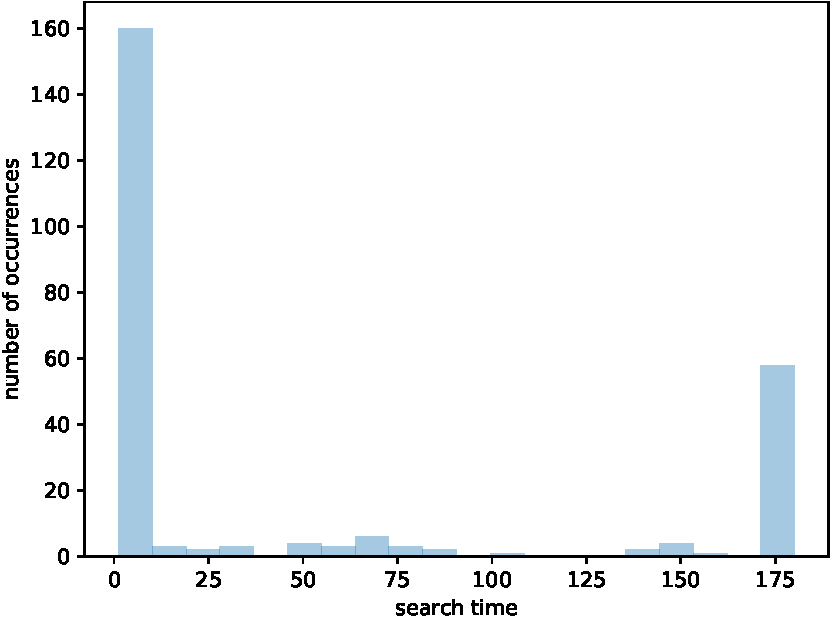
\includegraphics[width=0.6\textwidth]{histogram}
  \end{center}
 
  \caption{Histogram of search times (in seconds) in the benchmark.}
  \label{fig:histo}
\end{figure*}

\begin{figure*}[t!]
  \begin{center}
    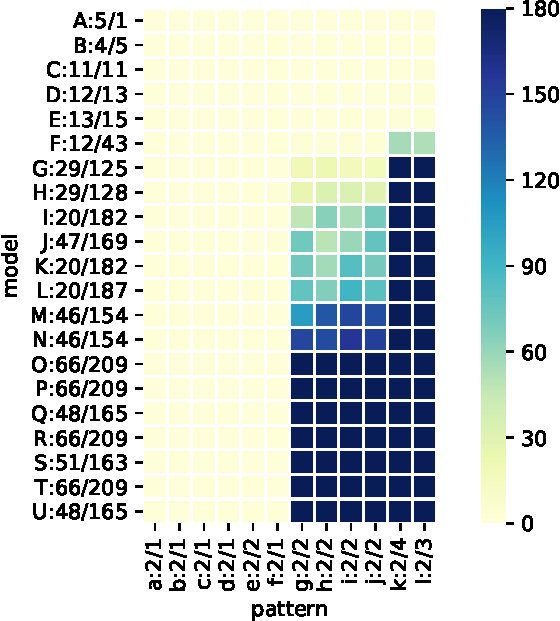
\includegraphics[width=0.6\textwidth]{heatmap}
  \end{center}
 % \vspace*{-1mm}
  \caption{Search times (in seconds) with respect to models and patterns. Models are indicated with an upper-case letter,  patterns with a lower-case letter.
 Model and pattern names are followed by pairs of numbers $e/r$: $e$ is the number of entities and $r$ the number of rules.}
  \label{fig:heatmap}
\end{figure*}

\begin{figure}[t]
\begin{small}
\begin{verbatim}
### reading 'pond.rr'
### 4 variables / 7 rules / 0 constraints
### reading 'pest.rr'
### 4 variables / 6 rules / 0 constraints
### building model
### running sat4j
... satisfiable [0:00:00.637612]
... objective function=2/24 [0:00:00.639101]
... objective function=4/24 [0:00:01.144709]
... objective function=6/24 [0:00:01.649645]
... optimum found
=== done running sat4j in 0:00:03.193784
*** OPTIMAL SAT => 6/24
### states
P+   ==>  Pe+
IF+  ==>  I+
Su+  ==>  R+
PF+  ==>  B+
### rules
R5: IF- >> PF-  ==>  R2: I- >> B-
R4: PF+ >> IF-  ==>  R1: B+ >> I-
R2: Su+ >> P-   ==>  R5: R+ >> Pe-
### normal exit
\end{verbatim}
\end{small}
\caption{A sample run of our prototype searching matches between the Pond and Pesticides models presented in Examples \ref{ex:pond} and \ref{ex:pests}.}
\label{fig:run}
\end{figure}


A more detailed view of this benchmark is provided in the ``heat-map'' depicted in Figure~\ref{fig:heatmap} that shows for each pattern and each model a color corresponding to the search time.
In this heat-map, models are named with an upper-case letter, and patterns with a lower-case letter; names are followed by pairs of numbers $e/r$ where $e$ is the number of entities and $r$ the number of rules in the model or pattern.
For instance, the ``prey-predator'' and ``live-in'' patterns we have presented in the introduction are \textsf{e} and \textsf{d} respectively.
Columns and rows have been sorted with respect to the sum of the values in the column and row, which allows to group larger search times in the lower-right corner.
From this plot we can draw the following observations:
%
\begin{itemize}
\item neither patterns nor models size seem to be the key factor that lead to the significant search time increase. For instance, models \textsf{S} and \textsf{J} have very similar sizes but do not yield similar search times. The same remark applies to patterns \textsf{e} and \textsf{g} to \textsf{j};
\item however, the shape of the heat-map shows that a key factor lies in patterns as pattern choice may yield a significant increase of search time, while increasing is more progressive with respect to model choice;
\item for toy models (\textsf{A} to \textsf{F} at the top), the solution is always quickly found;
\item for large, more detailed, models (\textsf{O} to \textsf{U} at the bottom), the pattern is the key factor to determine if a timeout occurs;
\item this is confirmed on intermediary models (\textsf{G} to \textsf{N} in the middle) where we can observe that more searches timeout as we go down the plot and, patterns all have the same size while models are not necessarily ordered by size.
\end{itemize}
%
So far, we have not identified what is the key factor that forbids a quick search.
For sure pattern size is a factor as we can see for patterns \textsf{k} and \textsf{l} (or models \textsf{O} to \textsf{U}), but what we observe from patterns \textsf{g}---\textsf{j} and models \textsf{F}---\textsf{L} shows that this is not the only aspect.
Considering our scoring function, search time is probably linked to the size of rules in the pattern and in the model, but this question will deserve further work to examine more in depths the characteristics of patterns that lead to these observed increasings of search times.



As a conclusion of this benchmark, we observe that searching a pattern in a model is always possible, usually in a very short time.
Moreover, in every case, a solution has been found quickly, which allows the user to interrupt the search very soon and yet get a match that is not optimal with respect to the scoring function but may be interesting already.
This is illustrated in Figure~\ref{fig:run} where we see how our prototype executes on the ecosystems from Examples \ref{ex:pond} and \ref{ex:pests}: it prints the values of the scoring function as soon as Sat4j finds them. At any time, it is possible to kill Sat4j which interrupts its computation and force it to print the best solution it has discovered so far.
It is interesting to note that this solution corresponds to none of those proposed in Example~\ref{ex:similarity} which are all matches that have been crafted manually and corresponded to our intuition about the two models. So, this shows that our method is able to propose something new, \ie something that a modeler would not necessarily imagine even on small examples.



A future extension of the implementation would be to enable re-injecting found matches in the PBO problem as negative constraints, in order to forbid the search to find them again. 
In addition, this would give a way to enumerate matches.  
It is indeed particularly relevant for ecologists to (automatically) identify several instances of the same interaction pattern (ecological processes) in the ecosystem dynamics under study. 

\section{Related work}
\label{sec:related}

The model of ecosystems developed in this paper is an instance of the more general family of rewriting systems \cite{Terese03}. 
Such systems have been shown convenient in formalizing models, in particular for systems biology and chemistry. 
In these domains, we thus find formalizations that are reminiscent of ours: the Biocham \cite{Fages:2008:FCB:1786698.1786702}, the $\kappa$-calculus \cite{DBLP:journals/tcs/DanosL04}, reaction systems \cite{reactionsystems}, activity networks 
\cite{toxico2017}, P-systems
\cite{DBLP:journals/ijfcs/PaunPRS11}
that describe the evolution of cells and/or molecules applying rewriting rules.


Yet, the question of similarity appears rather novel in rewriting systems. In a broader context, it is usually associated to the notion of equivalence. In concurrent systems like ours, equivalences are usually semantics based,  notable examples are partial ordering equivalences, trace equivalence \cite{vanglabbek89}, bisimulation \cite{Sangiorgi:2011:IBC:2103603}, principal transition sequences \cite{DBLP:conf/otm/WangHWWHS10}, etc.  
These notions are usually explored in theory and tailored to highly abstracted languages, moreover computed with a few existing tools. 
In practice, we cannot expect to use such approaches on the huge state spaces generated from detailed and realistic (qualitative) models of ecosystems.   

Works that are closer to ours can therefore be found in domains in which models use structural aspects rather than their behaviors. 
For instance in systems biology, several similarity measures can be found (a good survey summarizing the used techniques may be found in \cite{bbw090}).   
Technically speaking, these methods include the analysis of similar pathways through a structural approach, namely the search of t-invariants in Petri net models \cite{Baldan2013ComparingMP, DBLP:journals/topnoc/BaldanCGS13, Grafahrend-Belau2008}.
They also define a similarity score, but our goal and underlying model are considerably different.

Another domain that focuses on similarity rates is business process modeling. For instance in \cite{xiao}, the authors evaluate the similarity of Petri nets by comparing the set of structural elements such as places and transition arcs. Similarity is based on rates of identical elements. 
Instead, our approach is finer-grained and more flexible: the mappings allow different names of entities and rules, and we allow partially matched rules.  
In \cite{bae}, process-based models are studied and similarity is defined on sets of nodes as the proportion of matched ones. 
Yet, these authors do not deal with relations between them. Likewise, in \cite{DIJKMAN2011498},  other similarities are explored. In this context the authors still compare structural elements of workflows (\eg sets of nodes), but they allow different kinds of distance measures: string-edit distance, labels synonyms and contextual similarity. 
The latter measure is the closest to ours, as we consider separately the input (or conditions, the left hand side of a rule) and the output (realization, the right hand side of a rule) of a node.  
Conversely, here, we explicitly take into consideration penalties for elements that are not matched. 
The work in \cite{DIJKMAN2011498} shows how similarities in business process model are linked to the semantic web domain, a survey of which on corresponding metrics can be found in \cite{Euzenat}.   


Finally, concerning explicitly the pattern search, the work in \cite{Milo824} has analogous goals. These authors search for patterns by counting the number of occurrences of a given subgraph in 
specific networks (world wide web, electronic circuits, \dots) and comparing it to the number of occurrences in random generated networks.  
This approach is completely  different to ours, as their method applies to graphs while ours applies to  ``hyper-graphs". Moreover, they use techniques from statistics while we do not.









\section{\uppercase{Conclusion and perspectives}}
\label{sec:conclusion}

In this paper, we have presented a method for automatically comparing and assessing similarity between ecosystems defined as particular kinds of rewriting systems. 
We have defined a scoring function that takes into account not only the number of matching entities and rules, but also the quality of partial mappings between the left and right hand sides of rules. 
The approach has been successfully applied to the search of known interaction patterns (\ie ecological processes) in models of ecosystems. 

As a matter of fact this work represents a first step towards a more aware approach on ecosystem dynamics. 
The results we have obtained in our benchmark are promising: we quickly obtain optimal solutions for the vast majority of the cases studied. 
For the remaining ones, we obtain a solution that is not optimal in a short time, but we have no assessment of how far from optimal it is.
A possible option to solve this issue could be to add ecological information to assess the quality of a match (with a relevance score) closer to the modeler's expectations.  
In other words, a bigger match is not necessarily a better match. So far, our method searches for bigger matches. When the search is interrupted and yields a sub-optimal solution, a relevance score may help deciding whether it is already a ``good'' match or not.   
In practice, the matching of entities (here, ecosystemic entities) and rules (ecological processes) can be guided by adding additional constraints, such as to:  
 %CG attention aux termes : essayer de mettre partout les mêmes termes, par ex; choisir entre entities et agents, entre method et approach ... 
\begin{itemize}
 \item enforce the matching/identity between subsets of entities or rules. For example, if the model allows different categories of rules (each category possibly having a different semantics), the scoring function could be adapted to take into account this extension;  
 \item enforce the matching between entities/rules of the same category (for example match carnivores among them);
 \item diminish the importance of some entities/rules (\ie set a different weight for each matching up to forget some, if necessary).
 \end{itemize}

Finally, as a long term perspective, we may use our method to discover invariant patterns that are not known in advance, thus increasing the  understanding about ecosystem functioning. This could account for using our concept of similarity to identify matching parts of ecosystems and extract from those the new patterns. Experiments we have conducted so far in this direction showed bad performances as search time becomes prohibitive (as if we would have used patterns whose sizes are close to the studied models' sizes).  
However, sub-optimal patterns may provide interesting matches (which remains to be studied), or we may find a way to guide the search with respect to additional constraints (related to the previous idea of a relevance score). 





\section*{\uppercase{Acknowledgment}}
We would like to thank David Monniaux for his advise on MAXSAT and
PBO solvers, and Daniel Le Berre who has recommended Sat4j and has
been very helpful concerning its installation and use.


\bibliographystyle{apalike}
{\small

\bibliography{biblio}}
%

\end{document}